\documentclass[12pt,a4paper]{article}

%% ------------------------------------------------------------------
%% Packages
%% ------------------------------------------------------------------
\usepackage[utf8]{inputenc}
\usepackage[T1]{fontenc}
\usepackage[english]{babel}
\usepackage{geometry}
\usepackage{amsmath}
\usepackage{amssymb}
\usepackage{booktabs}
\usepackage{array}
\usepackage{longtable}
\usepackage{graphicx}
\usepackage{float}
\usepackage{caption}
\usepackage{subcaption}
\usepackage{hyperref}
\usepackage{xcolor}
\usepackage{listings}
\usepackage{parskip}
\usepackage{enumitem}
\usepackage{titlesec}
\usepackage{fancyhdr}
\usepackage{multirow}
\usepackage{makecell}

\geometry{
  top=2.5cm,
  bottom=2.5cm,
  left=3cm,
  right=3cm,
}

%% ------------------------------------------------------------------
%% Colors and hyperref
%% ------------------------------------------------------------------
\definecolor{linkblue}{RGB}{37,99,235}
\definecolor{codeblue}{RGB}{99,102,241}
\definecolor{codebg}{RGB}{248,250,252}
\definecolor{best}{RGB}{22,163,74}       % green for best values
\definecolor{secbest}{RGB}{234,88,12}    % orange for 2nd best

\hypersetup{
  colorlinks=true,
  linkcolor=linkblue,
  urlcolor=linkblue,
  citecolor=linkblue,
  pdftitle={Week 10: Recommendation, Ranking, and Decision Engine},
  pdfauthor={Grupo 06 --- Big Data},
}

%% ------------------------------------------------------------------
%% Code listings
%% ------------------------------------------------------------------
\lstset{
  basicstyle=\ttfamily\footnotesize,
  backgroundcolor=\color{codebg},
  frame=single,
  rulecolor=\color{gray!30},
  breaklines=true,
  columns=flexible,
  keywordstyle=\color{codeblue}\bfseries,
  commentstyle=\color{gray},
  stringstyle=\color{teal},
}

%% ------------------------------------------------------------------
%% Header / footer
%% ------------------------------------------------------------------
\pagestyle{fancy}
\fancyhf{}
\rhead{Grupo 06 --- Big Data}
\lhead{Week 10: Recommendation Engine}
\rfoot{\thepage}

%% ------------------------------------------------------------------
%% Title
%% ------------------------------------------------------------------
\title{
  \vspace{-1cm}
  \Large\textbf{Week 10 Milestone Report}\\[0.4em]
  \large Recommendation, Ranking, and Predictive Decision Engine\\[0.3em]
  \normalsize MovieLens Discovery System --- Semester Project
}
\author{
  Grupo 06 --- Big Data\\
  \texttt{BD-Grupo-06/movielens-discovery}
}
\date{\today}

%% ==================================================================
\begin{document}
%% ==================================================================

\maketitle
\thispagestyle{fancy}
\tableofcontents
\newpage

%% ------------------------------------------------------------------
\section{Executive Summary}
%% ------------------------------------------------------------------

This report covers Week~10 of the semester project: building a recommendation and ranking system
for the MovieLens~25M catalog. The work connects the technical infrastructure from Weeks~3, 5,
and~7 (ingestion, feature representation, and clustering) to a concrete decision task:
\emph{given a movie, which movies should be recommended next?}

Four systems were built and evaluated offline under two complementary protocols: a corrected
genre-relevance protocol over 4,994 query movies, and a Leave-One-Out (LOO) protocol over
10,000 user histories:

\begin{table}[H]
\centering
\small
\caption{System overview and primary evaluation results}
\begin{tabular}{llp{3.6cm}cc}
\toprule
\textbf{System} & \textbf{Type} & \textbf{Signal} & \textbf{\makecell{NDCG@10\\(genre, corrected)}} & \textbf{\makecell{Hit Rate@10\\(LOO)}} \\
\midrule
\texttt{popularity\_global}  & Baseline        & Raw rating-count popularity & 0.5852 & 0.0465 \\
\texttt{cluster\_popularity} & Hybrid baseline & Week~7 segmentation $\rightarrow$ Bayesian ranking & 0.5590 & --- (see Sec.~\ref{sec:loo}) \\
\texttt{content\_cosine}     & Baseline        & Cosine similarity on AE-13 embeddings & \textbf{0.9797} & 0.0368 \\
\texttt{svd\_collaborative}  & Advanced        & Item factors from Truncated SVD ($k=50$) & 0.8715 & \textbf{0.0795} \\
\bottomrule
\end{tabular}
\end{table}

The content-based cosine model dominates the genre-relevance protocol (NDCG@10 = 0.9797),
driven by the dense, genre-coherent structure of the Week~7 autoencoder embedding space.
Under the LOO protocol the ranking reverses: the SVD collaborative model is the strongest
\emph{predictive} system (Hit Rate@10 = 7.95\%). Two metric defects in the original genre
protocol (pool-denominator Recall and self-referential ideal DCG) were identified, documented,
and \textbf{corrected by recomputation} (\texttt{scripts/build\_week10\_eval\_corrected.py});
Section~\ref{sec:results} reports both the legacy and the corrected numbers for traceability.

%% ------------------------------------------------------------------
\section{Objective}
%% ------------------------------------------------------------------

The objective of Week~10 was to connect the prior technical layers to a concrete product decision:
\begin{quote}
  \textit{Given a seed movie, rank the catalog by relevance to that movie.}
\end{quote}

This is a \textbf{ranking and discovery system} (item-to-item), appropriate for catalog
discovery without a logged-in user context. Specific questions addressed:
\begin{itemize}[nosep]
  \item Does SVD collaborative filtering beat content-based similarity on genre-relevant recommendations?
  \item Where are the failure cases of each system?
  \item How does the Week~7 cluster layer support the recommendation layer?
\end{itemize}

%% ------------------------------------------------------------------
\section{Inputs and Reproducible Artifacts}
%% ------------------------------------------------------------------

\subsection{Input artifacts from previous weeks}

\begin{table}[H]
\centering
\caption{Inputs consumed from prior weeks}
\begin{tabular}{lll}
\toprule
\textbf{Artifact} & \textbf{Source} & \textbf{Purpose} \\
\midrule
\texttt{week07\_autoencoder\_embeddings\_latent\_13.parquet} & Week~7 & Content embedding (13-dim, 59,047 movies) \\
\texttt{week07\_kmeans\_assignments.csv} & Week~7 & Cluster-aware popularity ($k=7$) \\
\texttt{ratings\_clean.parquet} & Week~3 & SVD and popularity (25M ratings) \\
\texttt{movies\_catalog.parquet} & Week~3 & Metadata and genre labels (59,047 movies) \\
\bottomrule
\end{tabular}
\end{table}

\subsection{Week 10 output artifacts}

\begin{table}[H]
\centering
\caption{Output artifacts produced in Week~10 ($\approx$40\,MB total)}
\begin{tabular}{lll}
\toprule
\textbf{File} & \textbf{Description} & \textbf{Size} \\
\midrule
\texttt{week10\_popularity\_global.csv}    & Global Bayesian ranking (59,047 movies) & 4.8 MB \\
\texttt{week10\_popularity\_cluster.csv}   & Cluster-aware ranking                   & 5.1 MB \\
\texttt{week10\_content\_recs\_top20.parquet} & Content-based top-20 per query        & 0.6 MB \\
\texttt{week10\_svd\_item\_factors.parquet}   & SVD item factors (13,176 × 50)        & 2.8 MB \\
\texttt{week10\_svd\_recs\_top20.parquet}     & SVD collaborative top-20 per query    & 0.5 MB \\
\texttt{week10\_evaluation\_results.csv}   & Full metric comparison table            & 0.5 KB \\
\texttt{week10\_error\_analysis.csv}       & Strong and failure cases per system     & 2.4 KB \\
\texttt{week10\_evaluation\_summary.json}  & JSON summary of all evaluation results (includes LOO)  & 2.5 KB \\
\texttt{week10\_loo\_evaluation\_results.csv} & Leave-One-Out metric comparison table & 0.5 KB \\
\texttt{week10\_loo\_evaluation\_comparison.png} & LOO bar chart (Hit Rate, Precision, NDCG@K) & $\sim$90 KB \\
\texttt{week10\_genre\_eval\_corrected.csv} & Corrected genre-protocol metrics, 4 systems (incl.\ hybrid) & 1.2 KB \\
\texttt{week10\_data\_alignment.csv}       & Layer-by-layer data alignment for the hybrid claim & 0.5 KB \\
\bottomrule
\end{tabular}
\end{table}

\subsection{Week 10 scripts}

\begin{table}[H]
\centering
\caption{Scripts added in Week~10}
\begin{tabular}{lp{7.2cm}}
\toprule
\textbf{Script} & \textbf{Purpose} \\
\midrule
\texttt{scripts/build\_week10\_eval\_corrected.py} & Recomputes the genre evaluation with corrected Recall/NDCG, adds the \texttt{cluster\_popularity} hybrid, and emits the data-alignment table --- from committed artifacts only (no raw data needed) \\
\bottomrule
\end{tabular}
\end{table}

%% ------------------------------------------------------------------
\section{What Kind of System Is This?}
\label{sec:framing}
%% ------------------------------------------------------------------

Against the four candidate framings --- recommendation, ranking, prediction, or segmentation
feeding ranking --- this project is, precisely:

\begin{quote}
  \textbf{An item-to-item recommendation system, operationalized as a ranking task, with one
  variant that is segmentation feeding ranking, and a prediction-style evaluation.}
\end{quote}

\begin{table}[H]
\centering
\caption{Where each framing appears in this project}
\label{tab:framing}
\begin{tabular}{p{3.6cm}p{10.4cm}}
\toprule
\textbf{Framing} & \textbf{Where it appears in this project} \\
\midrule
\textbf{Recommendation} & The product task: given a seed movie, suggest movies (``You watched \emph{The Matrix}. You might also like\ldots''). Item-to-item, not user-to-item --- appropriate for cold-start catalog discovery with no logged-in user. \\
\textbf{Ranking} & The operationalization: every system outputs an \emph{ordered} top-20 list, and all evaluation metrics (Precision@K, NDCG@K, Hit Rate@K) are ranking metrics. \\
\textbf{Segmentation feeding ranking} & The \texttt{cluster\_popularity} hybrid: the Week~7 k-means segmentation ($k=7$) defines the candidate pool, and the Bayesian popularity score ranks within it. Section~\ref{subsec:hybrid_alignment} documents the data alignment this requires. \\
\textbf{Prediction} & The LOO evaluation (Section~\ref{sec:loo}) reframes the system as a predictive task: can it predict the \emph{next} movie a user actually rated? \\
\bottomrule
\end{tabular}
\end{table}

The primary identity is \textbf{recommendation via ranking}; segmentation (Week~7) feeds the
hybrid baseline; prediction is the lens of the second evaluation protocol, not the system's
design goal.

%% ------------------------------------------------------------------
\section{Baseline Systems}
%% ------------------------------------------------------------------

\subsection{Global popularity baseline}

Every movie is ranked by its Bayesian-adjusted score:

\begin{equation}
  \text{bayesian\_score} = \frac{C \cdot \mu + n \cdot \bar{r}}{C + n}
\end{equation}

\textbf{Parameters}: global mean $\mu = 3.0714$, prior count $C = 1.0$ (10th percentile of rating counts).

\textbf{Note on the evaluated list.}
The published artifact \texttt{week10\_popularity\_global.csv} ranks by
\texttt{bayesian\_score}, but the static top-20 list used in the genre evaluation ranks by
\textbf{raw rating count} (most-rated movies). Both are reported here for transparency;
the reproduction check in \texttt{build\_week10\_eval\_corrected.py} confirms the
rating-count list is the one behind the published metrics
(max abs.\ difference 0.0002 vs the original run).

The catalog has a strong long-tail: 59,047 movies, but fewer than 5\% have more than
10,000 ratings, as shown in Figure~\ref{fig:pop_dist}.

\begin{figure}[H]
  \centering
  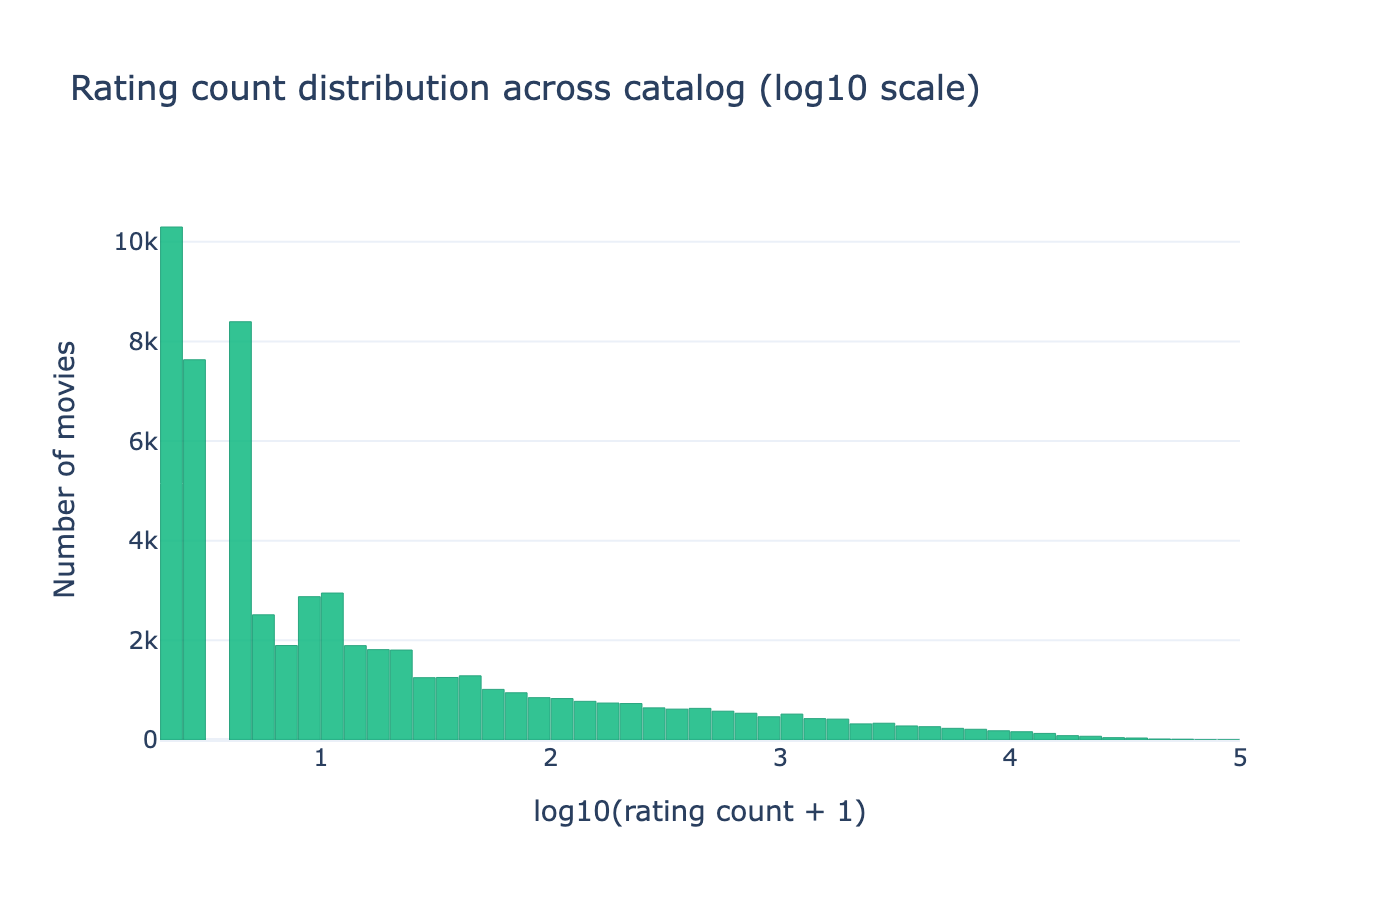
\includegraphics[width=0.85\textwidth]{../../artifacts/week10/week10_popularity_distribution.png}
  \caption{Rating count distribution across the catalog (log10 scale).
  The long-tail structure motivates the Bayesian adjustment: most movies have fewer than 100 ratings.}
  \label{fig:pop_dist}
\end{figure}

\subsection{Cluster-aware popularity baseline}

Restricts the ranking to movies within the same Week~7 cluster as the query movie.
Table~\ref{tab:cluster_stats} shows the cluster engagement disparity:
Cluster~4 (23,093 movies, mean 9.1 ratings each) represents the low-engagement catalog tail,
while Cluster~0 averages 1,666 ratings per movie.

\begin{table}[H]
\centering
\caption{Cluster-level popularity statistics}
\label{tab:cluster_stats}
\begin{tabular}{rrrrr}
\toprule
\textbf{Cluster} & \textbf{Movies} & \textbf{Mean rating count} & \textbf{Mean avg. rating} & \textbf{Mean Bayesian score} \\
\midrule
0 & 9,363  & 1,665.9 & 3.291 & 3.288 \\
1 & 2,650  &   505.1 & 3.130 & 3.152 \\
2 & 5,013  &   327.6 & 3.064 & 3.091 \\
3 & 10,036 &   463.6 & 2.739 & 2.815 \\
4 & 23,093 &     9.1 & 3.042 & 3.061 \\
5 & 5,346  &    55.4 & 3.383 & 3.321 \\
6 & 3,546  &   356.1 & 3.121 & 3.126 \\
\bottomrule
\end{tabular}
\end{table}

\begin{figure}[H]
  \centering
  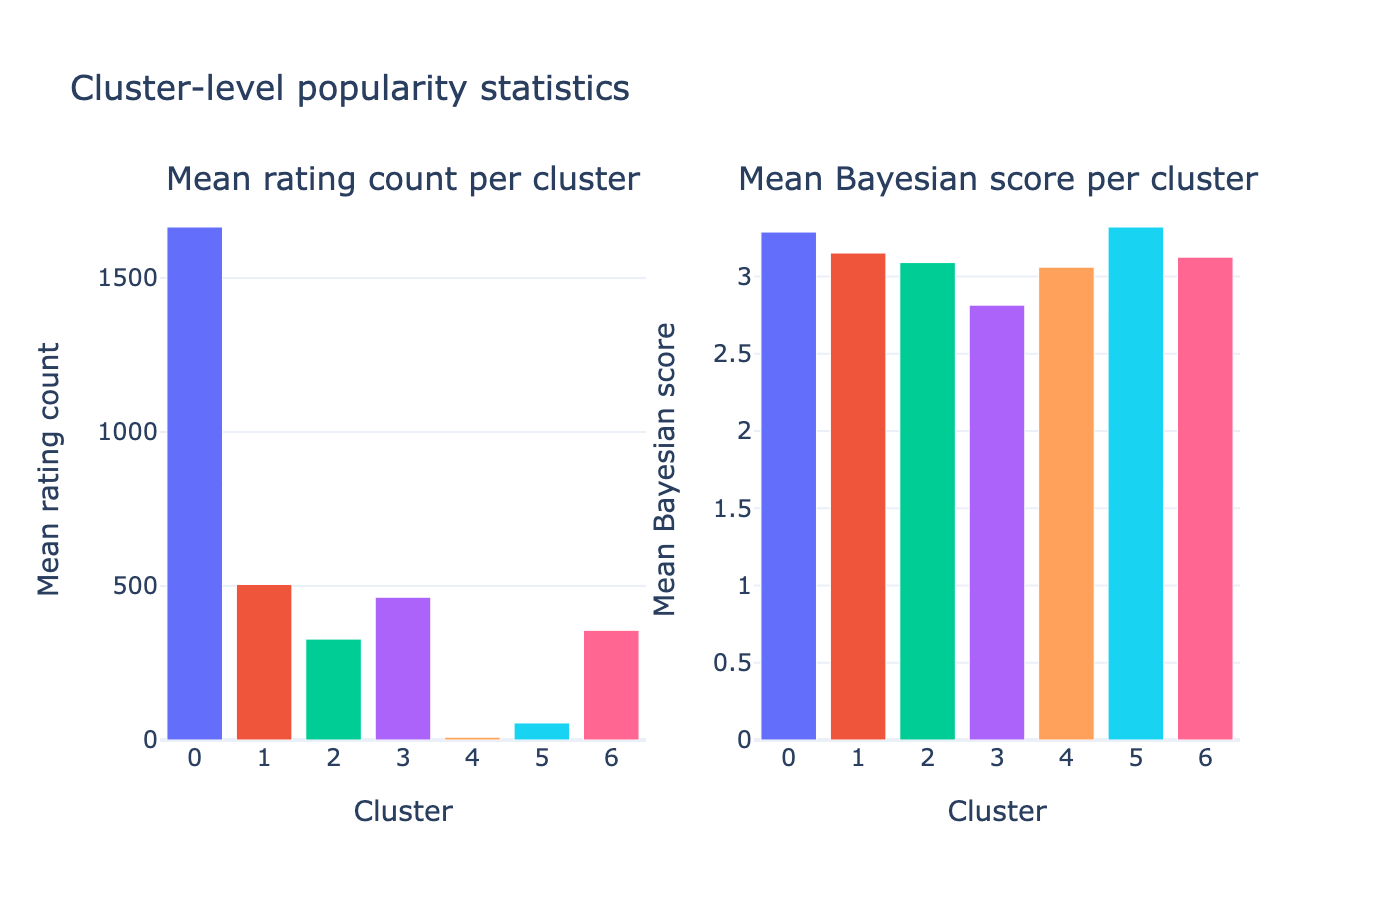
\includegraphics[width=0.95\textwidth]{../../artifacts/week10/week10_cluster_popularity_stats.png}
  \caption{Mean rating count and Bayesian score per Week~7 cluster.
  Cluster~0 (mainstream Drama/Comedy) dominates engagement; Cluster~4 (long-tail catalog) is minimal.}
  \label{fig:cluster_pop}
\end{figure}

This hybrid is evaluated alongside the other three systems in
Section~\ref{subsec:corrected_table}.

\subsection{Hybrid claim and data alignment}
\label{subsec:hybrid_alignment}

\texttt{cluster\_popularity} is a \textbf{hybrid system}: an unsupervised \emph{content}
segmentation (Week~7 k-means over autoencoder embeddings of Week~5 content/behavioral
features) feeding a \emph{behavioral} popularity ranking (Week~3 ratings). A hybrid is only
valid if the layers actually join --- Table~\ref{tab:data_alignment} documents the alignment,
all on the \texttt{movieId} key
(source: \texttt{artifacts/week10/week10\_data\_alignment.csv}).

\begin{table}[H]
\centering
\small
\caption{Layer-by-layer data alignment for the hybrid claim}
\label{tab:data_alignment}
\begin{tabular}{p{6.8cm}lrr}
\toprule
\textbf{Layer} & \textbf{Join key} & \textbf{Movies} & \textbf{Catalog coverage} \\
\midrule
\texttt{movies\_catalog} (Week~3)                          & movieId & 62,423 & 100.00\% \\
Autoencoder embeddings AE-13 (Week~7)                      & movieId & 62,423 & 100.00\% \\
K-means assignments, $k=7$ (Week~7)                        & movieId & 62,423 & 100.00\% \\
Rated movies with genres = evaluation universe (Week~10)   & movieId & 59,047 & 94.59\% \\
Cluster popularity ranking (Week~10 hybrid)                & movieId & 59,047 & 94.59\% \\
SVD item factors (Week~10)                                 & movieId & 13,176 & 21.11\% \\
Query set, content/SVD (Week~10)                           & movieId &  5,000 & 8.01\% \\
Evaluated queries (intersection, with genres)              & movieId &  4,994 & 8.00\% \\
\bottomrule
\end{tabular}
\end{table}

Where rows drop, and why:
\begin{itemize}[nosep]
  \item \textbf{62,423 $\rightarrow$ 59,047}: movies with zero ratings have no popularity
    signal and leave the evaluation universe. Every rated movie has a cluster assignment,
    so the hybrid join loses nothing beyond unrated movies.
  \item \textbf{59,047 $\rightarrow$ 13,176}: the SVD filter ($\geq 50$ ratings/movie) ---
    a coverage limitation of the collaborative system, not of the hybrid.
  \item \textbf{5,000 $\rightarrow$ 4,994}: the evaluation intersects the content and SVD
    query sets and requires at least one genre label, leaving exactly \textbf{4,994} queries
    (this resolves the 4,994 vs 4,999 count discrepancy between earlier artifact versions:
    4,999 was counted before the intersection).
\end{itemize}

%% ------------------------------------------------------------------
\section{Content-Based Baseline}
%% ------------------------------------------------------------------

\subsection{Method}

Top-20 most similar movies are retrieved using cosine similarity over the
13-dimensional autoencoder embedding space from Week~7:

\begin{equation}
  \text{sim}(i, j) = \frac{\mathbf{e}_i \cdot \mathbf{e}_j}{\|\mathbf{e}_i\| \cdot \|\mathbf{e}_j\|}
\end{equation}

Embedding rows are L2-normalized before retrieval (dot product = cosine similarity).

\subsection{Similarity distribution}

\begin{figure}[H]
  \centering
  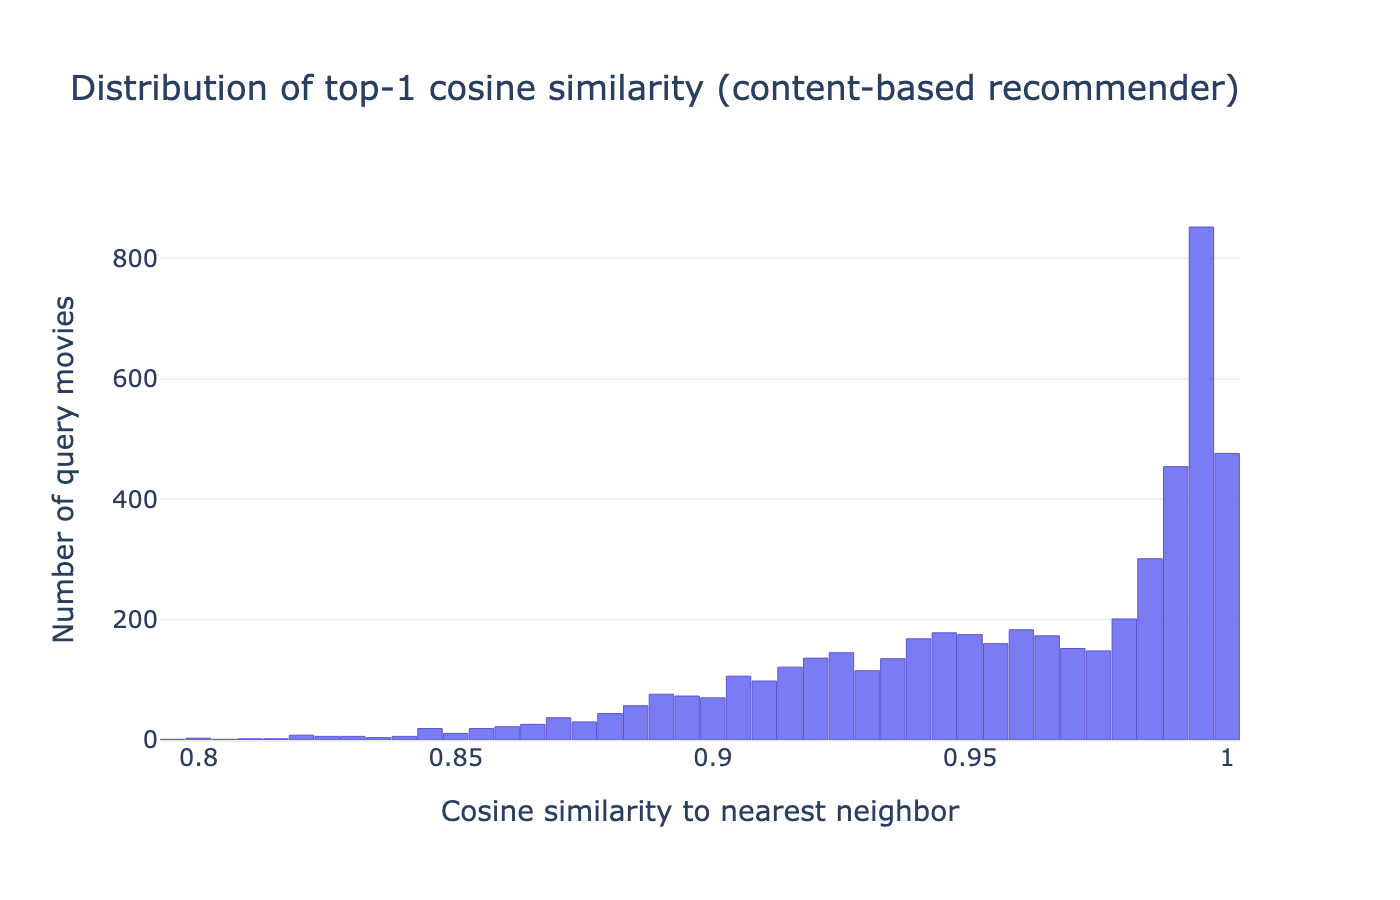
\includegraphics[width=0.80\textwidth]{../../artifacts/week10/week10_cosine_similarity_dist.png}
  \caption{Distribution of top-1 cosine similarity (nearest neighbor) across 5,000 query movies.
  The concentration near 1.0 confirms the autoencoder learned a dense, genre-coherent embedding space.}
  \label{fig:cosine_dist}
\end{figure}

%% ------------------------------------------------------------------
\section{Advanced System: SVD Collaborative Filtering}
%% ------------------------------------------------------------------

\subsection{Model design}

The advanced system factorizes the mean-centered user-item rating matrix:

\begin{equation}
  \mathbf{R}_{\text{centered}} \approx \mathbf{U} \boldsymbol{\Sigma} \mathbf{V}^\top
\end{equation}

\textbf{Matrix}: 162,540 users $\times$ 13,176 movies (after filtering: $\geq50$ ratings/movie,
$\geq20$ ratings/user). \textbf{Density}: 1.15\%. \textbf{Centering}: per-user mean subtraction.
\textbf{Latent factors}: $k=50$, chosen from the sweep below.

Recommendations use cosine similarity between L2-normalized rows of $\mathbf{V}$
(item factor vectors), capturing behavioral co-occurrence patterns.

\subsection{Latent factor sweep}

\begin{table}[H]
\centering
\caption{SVD latent factor sweep results}
\label{tab:svd_sweep}
\begin{tabular}{rrl}
\toprule
\textbf{Components} & \textbf{Explained variance} & \textbf{Time (s)} \\
\midrule
10  &  9.33\% & 1.35 \\
20  & 12.27\% & 2.11 \\
30  & 14.42\% & 2.07 \\
\textbf{50}  & \textbf{17.79\%} & \textbf{2.83} \\
75  & 21.11\% & 3.57 \\
100 & 23.89\% & 4.60 \\
150 & 28.58\% & 5.37 \\
\bottomrule
\end{tabular}
\end{table}

$k=50$ was selected: the variance curve flattens past this point with diminishing returns
(Figure~\ref{fig:svd_sweep}).

\begin{figure}[H]
  \centering
  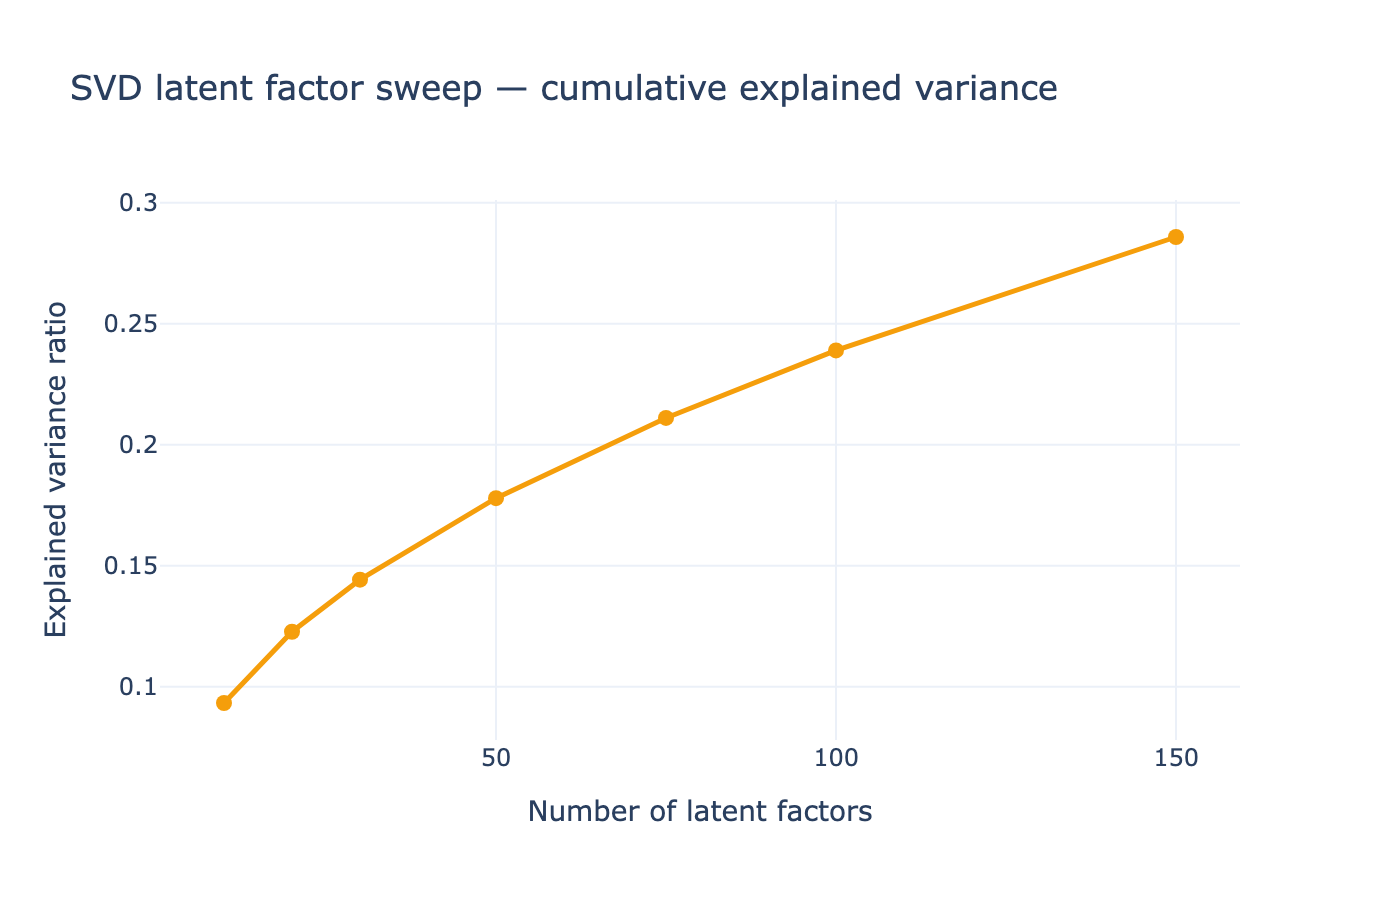
\includegraphics[width=0.80\textwidth]{../../artifacts/week10/week10_svd_sweep.png}
  \caption{SVD cumulative explained variance vs.\ number of components.
  The elbow appears near $k=50$.}
  \label{fig:svd_sweep}
\end{figure}

\subsection{Singular value spectrum}

The first singular value $\sigma_1 = 996$ is approximately twice the second $\sigma_2 = 519$,
confirming fast decay and strong low-rank structure in the rating matrix ---
a favorable property for collaborative filtering.

\begin{figure}[H]
  \centering
  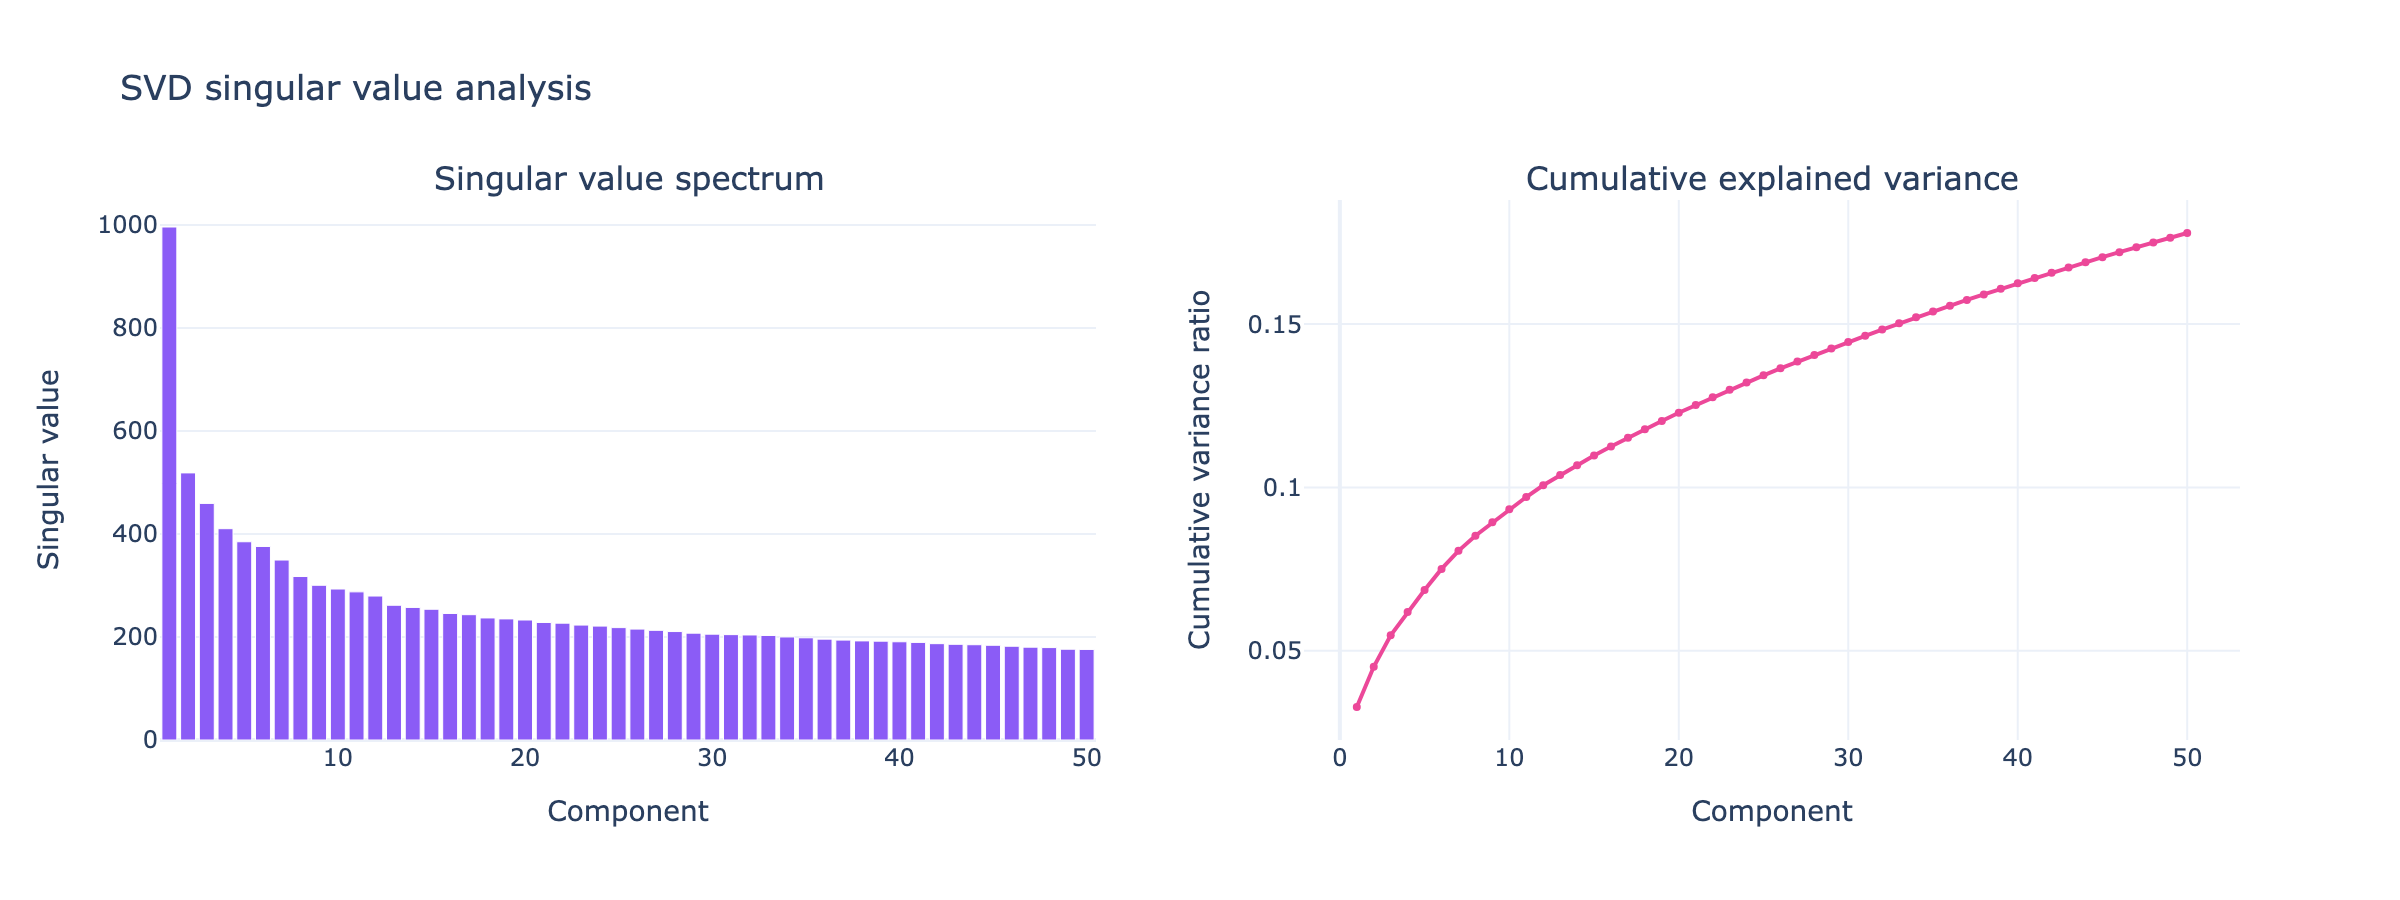
\includegraphics[width=0.95\textwidth]{../../artifacts/week10/week10_svd_singular_values.png}
  \caption{Left: singular value spectrum (first 50 components). Right: cumulative explained variance.
  Fast decay confirms the matrix has substantial low-rank structure.}
  \label{fig:sv_spectrum}
\end{figure}

\subsection{SVD score distribution}

\begin{figure}[H]
  \centering
  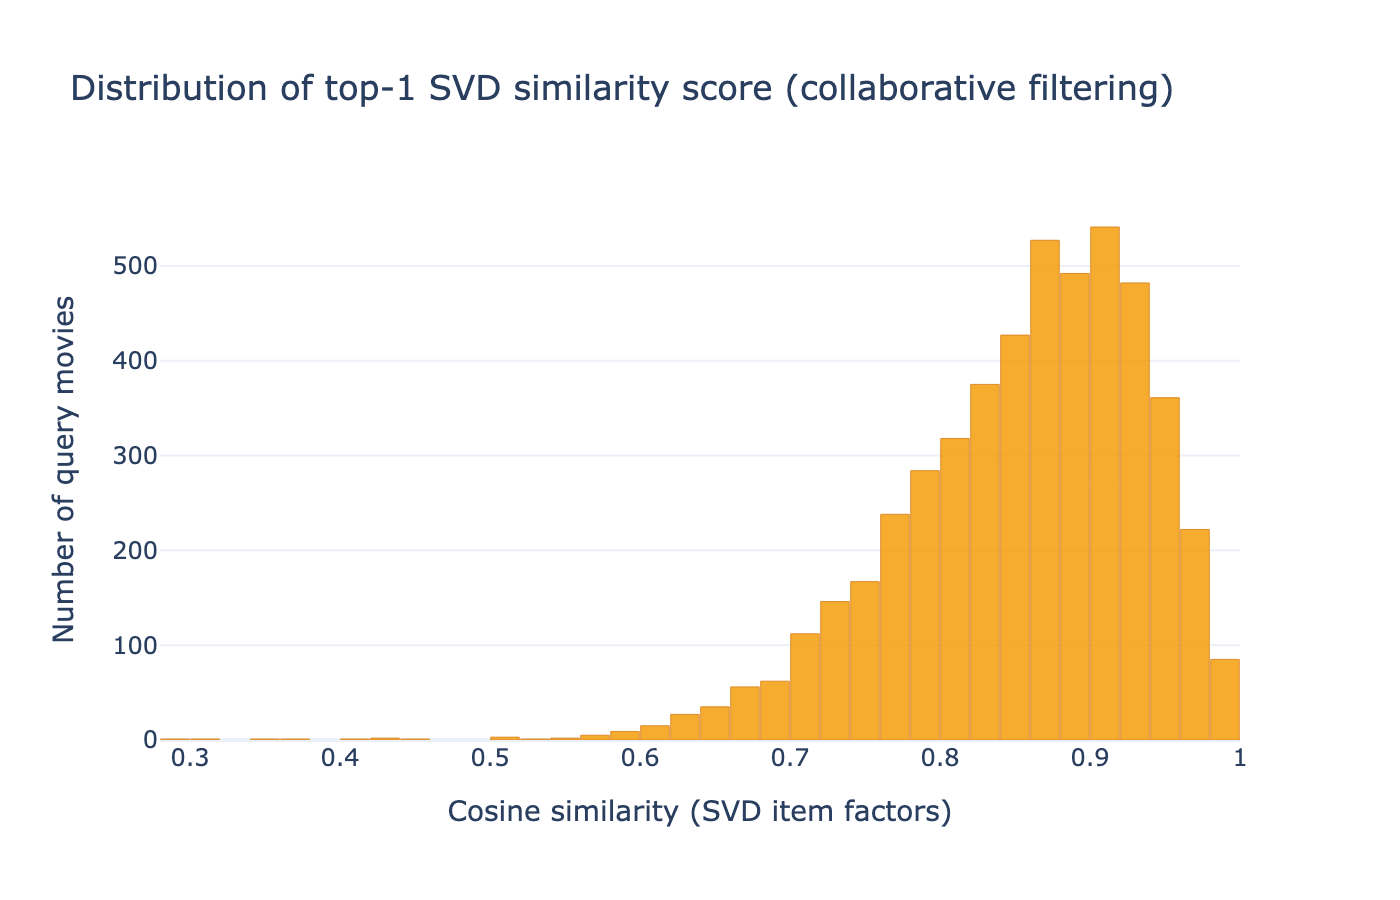
\includegraphics[width=0.80\textwidth]{../../artifacts/week10/week10_svd_score_dist.png}
  \caption{Distribution of top-1 SVD similarity scores across 5,000 query movies.
  Scores are concentrated at higher values than content-based similarity,
  reflecting tight co-occurrence structure among popular films.}
  \label{fig:svd_score_dist}
\end{figure}

%% ------------------------------------------------------------------
\section{Offline Evaluation Protocol}
%% ------------------------------------------------------------------

\subsection{Setup}

\begin{itemize}[nosep]
  \item \textbf{Evaluation universe}: the 59,047 rated movies with genre labels (movies with
    zero ratings carry no signal for any system and are excluded)
  \item \textbf{Query movies}: exactly \textbf{4,994} --- the intersection of the content and
    SVD query sets (5,000 most-rated movies each), restricted to queries with at least one
    genre label
  \item \textbf{Recommendation lists}: top-20 per system per query (the query itself is
    always excluded)
  \item \textbf{Relevance criterion}: a recommendation is relevant if it shares
    \textbf{at least one genre} with the query
\end{itemize}

\subsection{Relevance criterion}
\label{subsec:relevance}

\begin{equation}
  \text{relevant}(i, j) =
  \begin{cases}
    1 & \text{if } G_i \cap G_j \neq \emptyset \\
    0 & \text{otherwise}
  \end{cases}
\end{equation}

Genre overlap is a reproducible, catalog-level proxy requiring no user ground truth.
It favors content methods by construction; a user-history holdout is stronger
(see Section~\ref{sec:loo} for the Leave-One-Out evaluation added after review).

\textbf{Recall@$K$ and NDCG@$K$ corrections.}
In the original run, the \texttt{Recall@K} denominator was the number of relevant items
within the system's own top-20 pool --- not the full universe --- which inflated Recall
artificially (e.g.\ \texttt{content\_cosine} Recall@20 $= 0.9994$). The ideal DCG in
\texttt{NDCG@K} had the same self-referential defect (it was built from the relevant count
inside the retrieved top-$K$). Both defects are documented in the evaluation notebook
\textbf{and corrected by recomputation} in \texttt{scripts/build\_week10\_eval\_corrected.py},
which first reproduces the original numbers (max abs.\ difference 0.0002) and then recomputes
\texttt{catalog\_recall\_at\_k} (denominator = genre-relevant movies in the full universe;
on average \textbf{22,301} per query) and \texttt{ndcg\_at\_k\_corrected} (ideal DCG = $K$
relevant items). Section~\ref{subsec:legacy_table} keeps the legacy table for traceability;
Section~\ref{subsec:corrected_table} reports the corrected metrics. The LOO evaluation in
Section~\ref{sec:loo} additionally provides a Recall that is correct by construction.

\subsection{Metrics}
\label{subsec:metrics}

\begin{table}[H]
\centering
\caption{Evaluation metrics}
\begin{tabular}{lp{10.5cm}}
\toprule
\textbf{Metric} & \textbf{Definition} \\
\midrule
Precision@$K$ & $\frac{1}{K}\sum_{k=1}^{K} \mathbf{1}[\text{rec}_k \text{ relevant}]$ \\[4pt]
Recall@$K$ & Fraction of genre-relevant items retrieved in top-$K$.
  \emph{Legacy version (Sec.~\ref{subsec:legacy_table})}: denominator = relevant items in the
  system's own pool (inflated).
  \emph{Corrected version (Sec.~\ref{subsec:corrected_table})}: denominator = relevant items
  in the full universe \\[4pt]
NDCG@$K$ & Normalized Discounted Cumulative Gain --- position-weighted relevance.
  \emph{Corrected version}: ideal DCG assumes $K$ relevant items \\[4pt]
Hit Rate@$K$ & $\mathbf{1}[\exists\, k \leq K : \text{rec}_k \text{ relevant}]$ \\
\bottomrule
\end{tabular}
\end{table}

With $\sim$22,301 relevant movies per query and only 20 recommendations, corrected catalog
Recall is structurally tiny ($\leq 20/22{,}301 \approx 0.0009$ on average) for \emph{any}
system; \textbf{Precision@$K$ and NDCG@$K$ are the informative metrics under this protocol},
and Recall is meaningfully measured only in the LOO protocol.

\subsection{Candidate-pool definition}
\label{subsec:candidate_pools}

The rubric requires an explicit candidate-pool definition --- what each system is allowed to
rank from, per protocol:

\begin{table}[H]
\centering
\small
\caption{Candidate pools per system and protocol}
\label{tab:candidate_pools}
\begin{tabular}{p{3.4cm}p{5.4cm}p{5.0cm}}
\toprule
\textbf{System} & \textbf{Genre protocol (item-to-item)} & \textbf{LOO protocol (user histories)} \\
\midrule
\texttt{popularity\_global} & Static global list: top-20 movies by raw rating count, minus the query & Top-500 most-rated movies in the LOO training split, minus the user's seen movies \\
\texttt{cluster\_popularity} & Movies in the query's Week~7 cluster ($k=7$), ranked by Bayesian score, minus the query & Not evaluated (see Sec.~\ref{sec:loo}) \\
\texttt{content\_cosine} & All 59,047 rated movies with AE-13 embeddings, minus the query & The 13,176 SVD-factored movies, minus the user's seen movies \\
\texttt{svd\_collaborative} & The 13,176 movies in the filtered SVD matrix ($\geq 50$ ratings), minus the query & The 13,176 SVD-factored movies, minus the user's seen movies \\
\bottomrule
\end{tabular}
\end{table}

Two asymmetries are deliberate and disclosed: (a) in the genre protocol,
\texttt{svd\_collaborative} can only recommend from 22.3\% of the catalog (its training
filter), while \texttt{content\_cosine} ranks the full rated universe; (b) in the LOO
protocol, only the 9,885 of 10,000 sampled users whose held-out movie is inside the
13,176-movie factor space are scoreable for the content and SVD systems
($n_{\text{queries}} = 10{,}000$ for popularity, 9,885 for the other two).

%% ------------------------------------------------------------------
\section{Evaluation Results}
\label{sec:results}
%% ------------------------------------------------------------------

\subsection{Legacy metric table (original run --- Recall and NDCG inflated, kept for traceability)}
\label{subsec:legacy_table}

Table~\ref{tab:eval_results} presents the metrics from the original run at $K \in \{5, 10, 20\}$.

\begin{table}[H]
\centering
\caption{Legacy offline evaluation results — genre-relevance protocol, $n_{\text{queries}} = 4{,}994$}
\label{tab:eval_results}
\begin{tabular}{llcccc}
\toprule
\textbf{System} & \textbf{K} & \textbf{Precision@K} & \textbf{\makecell{Recall@K\\(pool, inflated)}} & \textbf{\makecell{NDCG@K\\(legacy)}} & \textbf{Hit Rate@K} \\
\midrule
\multirow{3}{*}{popularity\_global}
  & 5  & 0.5820 & 0.3621 & 0.8437 & 0.9553 \\
  & 10 & 0.5554 & 0.6089 & 0.8390 & 0.9720 \\
  & 20 & 0.4593 & 0.9808 & 0.8206 & 0.9808 \\
\midrule
\multirow{3}{*}{content\_cosine}
  & 5  & 0.9822 & 0.2535 & 0.9930 & 0.9982 \\
  & 10 & 0.9775 & 0.5032 & 0.9925 & 0.9990 \\
  & 20 & 0.9722 & 0.9994 & 0.9916 & 0.9994 \\
\midrule
\multirow{3}{*}{svd\_collaborative}
  & 5  & 0.8807 & 0.2656 & 0.9525 & 0.9890 \\
  & 10 & 0.8603 & 0.5155 & 0.9496 & 0.9958 \\
  & 20 & 0.8379 & 0.9986 & 0.9462 & 0.9986 \\
\bottomrule
\end{tabular}
\end{table}

Source: \texttt{artifacts/week10/week10\_evaluation\_results.csv}
($n_{\text{queries}} = 4{,}994$). The Recall and NDCG columns carry the self-referential
defects described in Section~\ref{subsec:relevance}; read the corrected table below instead.

\subsection{Corrected metric table (all four systems, including the hybrid)}
\label{subsec:corrected_table}

\begin{table}[H]
\centering
\caption{Corrected offline evaluation results — genre-relevance protocol, $n_{\text{queries}} = 4{,}994$}
\label{tab:eval_corrected}
\begin{tabular}{llcccc}
\toprule
\textbf{System} & \textbf{K} & \textbf{Precision@K} & \textbf{\makecell{Catalog\\Recall@K}} & \textbf{\makecell{NDCG@K\\(corrected)}} & \textbf{Hit Rate@K} \\
\midrule
\multirow{3}{*}{popularity\_global}
  & 5  & 0.5820 & 0.000136 & 0.6207 & 0.9553 \\
  & 10 & 0.5554 & 0.000263 & 0.5852 & 0.9720 \\
  & 20 & 0.4595 & 0.000455 & 0.5062 & 0.9808 \\
\midrule
\multirow{3}{*}{cluster\_popularity}
  & 5  & 0.5479 & 0.000151 & 0.5731 & 0.8104 \\
  & 10 & 0.5449 & 0.000297 & 0.5590 & 0.8214 \\
  & 20 & 0.5784 & 0.000634 & 0.5762 & 0.9864 \\
\midrule
\multirow{3}{*}{content\_cosine}
  & 5  & \textbf{0.9822} & \textbf{0.000296} & \textbf{0.9834} & \textbf{0.9982} \\
  & 10 & \textbf{0.9775} & \textbf{0.000588} & \textbf{0.9797} & \textbf{0.9990} \\
  & 20 & \textbf{0.9722} & \textbf{0.001168} & \textbf{0.9753} & \textbf{0.9994} \\
\midrule
\multirow{3}{*}{svd\_collaborative}
  & 5  & 0.8807 & 0.000251 & 0.8882 & 0.9890 \\
  & 10 & 0.8603 & 0.000485 & 0.8715 & 0.9958 \\
  & 20 & 0.8379 & 0.000934 & 0.8519 & 0.9986 \\
\bottomrule
\end{tabular}
\end{table}

\textbf{Best values per column and $K$ are bolded} --- \texttt{content\_cosine} leads every
column. Source: \texttt{artifacts/week10/week10\_genre\_eval\_corrected.csv}
($n_{\text{queries}} = 4{,}994$). Catalog Recall is structurally tiny under this protocol
(Section~\ref{subsec:metrics}) and is shown for completeness, not comparison against the
legacy column.

\paragraph{Key finding.} \texttt{content\_cosine} still dominates after correction. Its
Precision@5 of 0.982 means 49 out of every 50 recommendations at rank 1--5 share at least one
genre with the query --- a direct consequence of the genre-coherent Week~7 autoencoder space.
The correction's largest effect is on \texttt{popularity\_global}: its legacy NDCG@10 of 0.839
drops to 0.585 once the ideal DCG stops adapting to the system's own output.

\paragraph{Hybrid finding.} \texttt{cluster\_popularity} trades coverage for depth.
Restricting candidates to the query's Week~7 cluster \emph{lowers} Hit Rate@10 (0.821 vs
0.972 global --- niche queries can land in clusters whose popular movies don't share their
genres), but its precision barely decays with depth (0.548 $\rightarrow$ 0.578 from $K=5$ to
$K=20$) while the global list collapses (0.582 $\rightarrow$ 0.460). At $K=20$ the hybrid is
the \textbf{more precise popularity baseline}, confirming the Week~7 segmentation contributes
real signal --- segmentation feeding ranking, as claimed in Section~\ref{sec:framing}.

\subsection{Multi-metric comparison chart}

The charts in this and the following two subsections were rendered from the original (legacy)
run and therefore show the pre-correction Recall/NDCG values for the three original systems;
the corrected numbers are in Table~\ref{tab:eval_corrected}.

\begin{figure}[H]
  \centering
  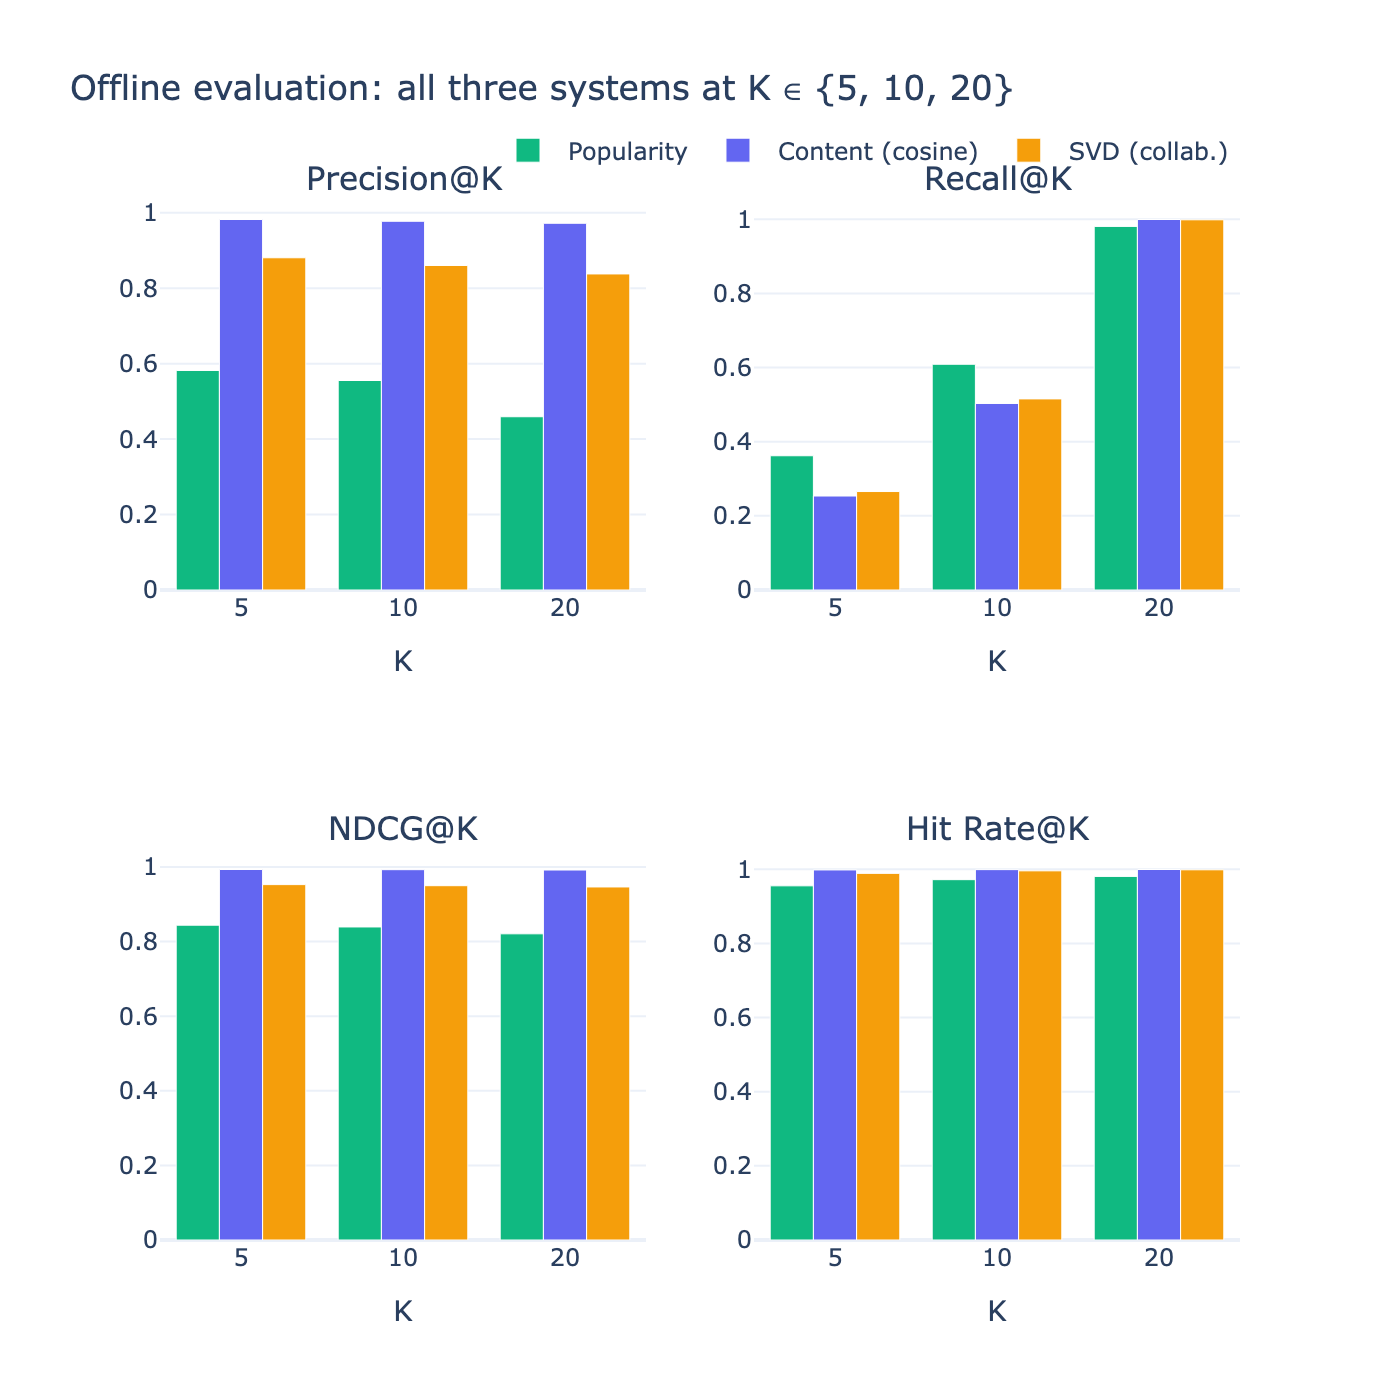
\includegraphics[width=\textwidth]{../../artifacts/week10/week10_evaluation_comparison.png}
  \caption{All four metrics for all three systems at $K \in \{5, 10, 20\}$.
  Content cosine (violet) dominates on Precision and NDCG.
  SVD collaborative (amber) beats popularity (green) on all metrics.}
  \label{fig:eval_comparison}
\end{figure}

\subsection{NDCG@10 summary}

\begin{figure}[H]
  \centering
  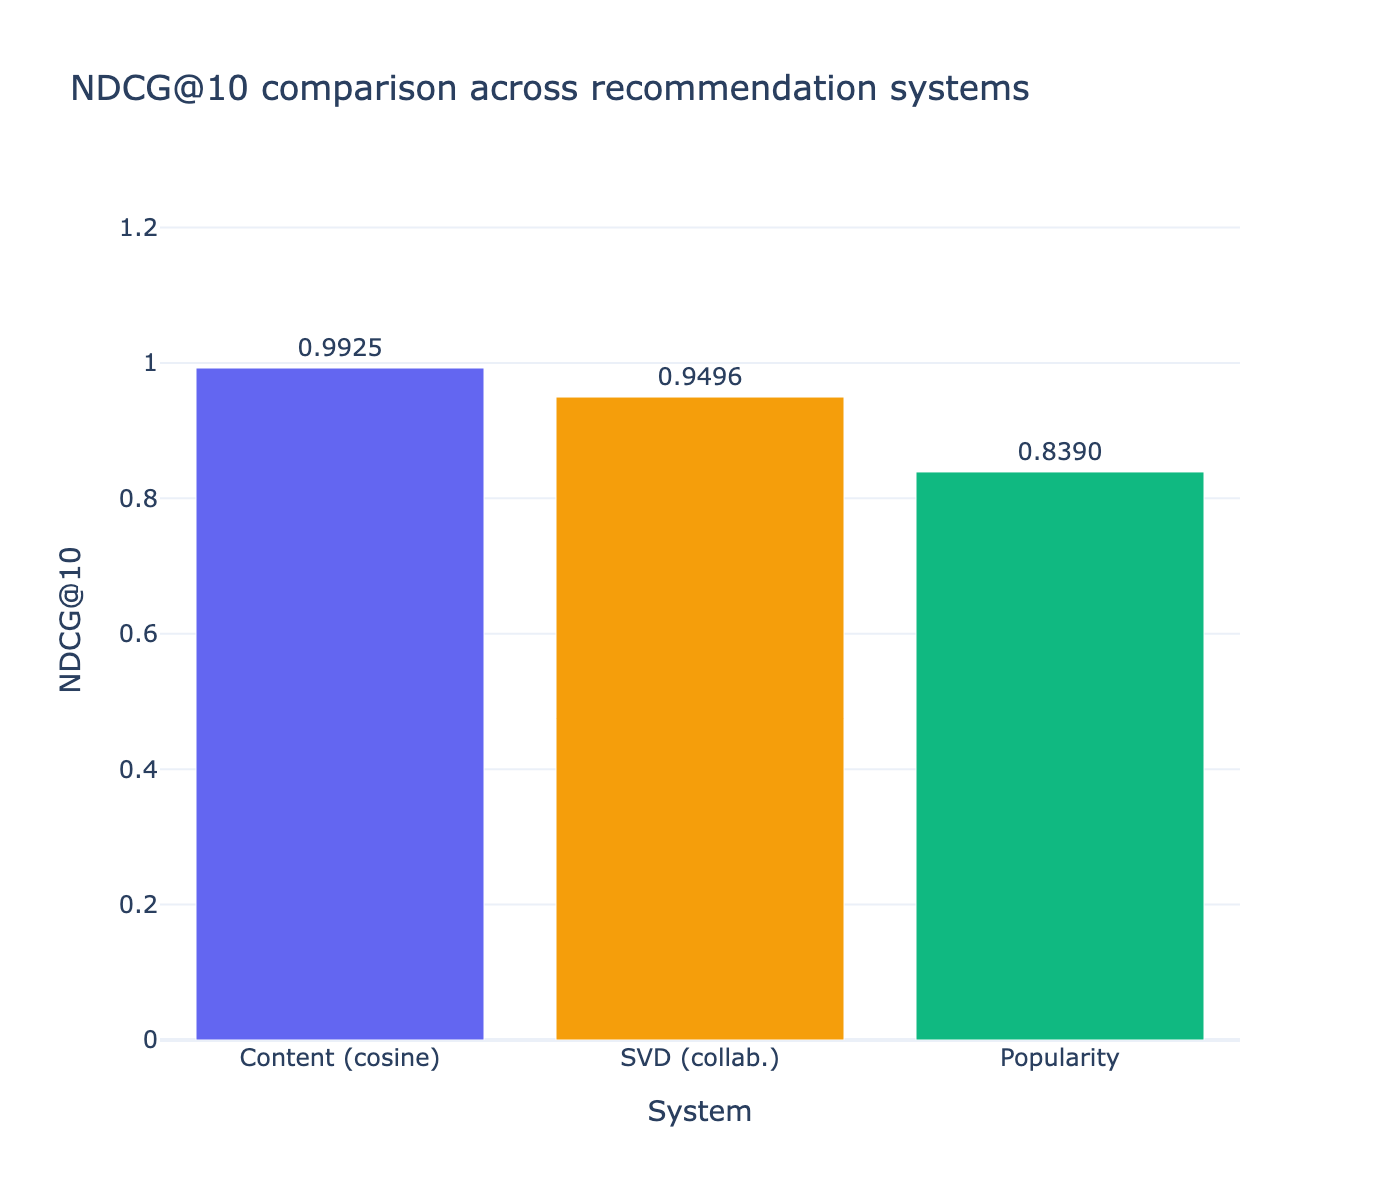
\includegraphics[width=0.70\textwidth]{../../artifacts/week10/week10_ndcg10_comparison.png}
  \caption{NDCG@10 for the three systems. Content cosine achieves 0.9925,
  SVD collaborative 0.9496, and popularity global 0.8390.}
  \label{fig:ndcg10}
\end{figure}

\subsection{Per-query NDCG@10 distribution}

\begin{figure}[H]
  \centering
  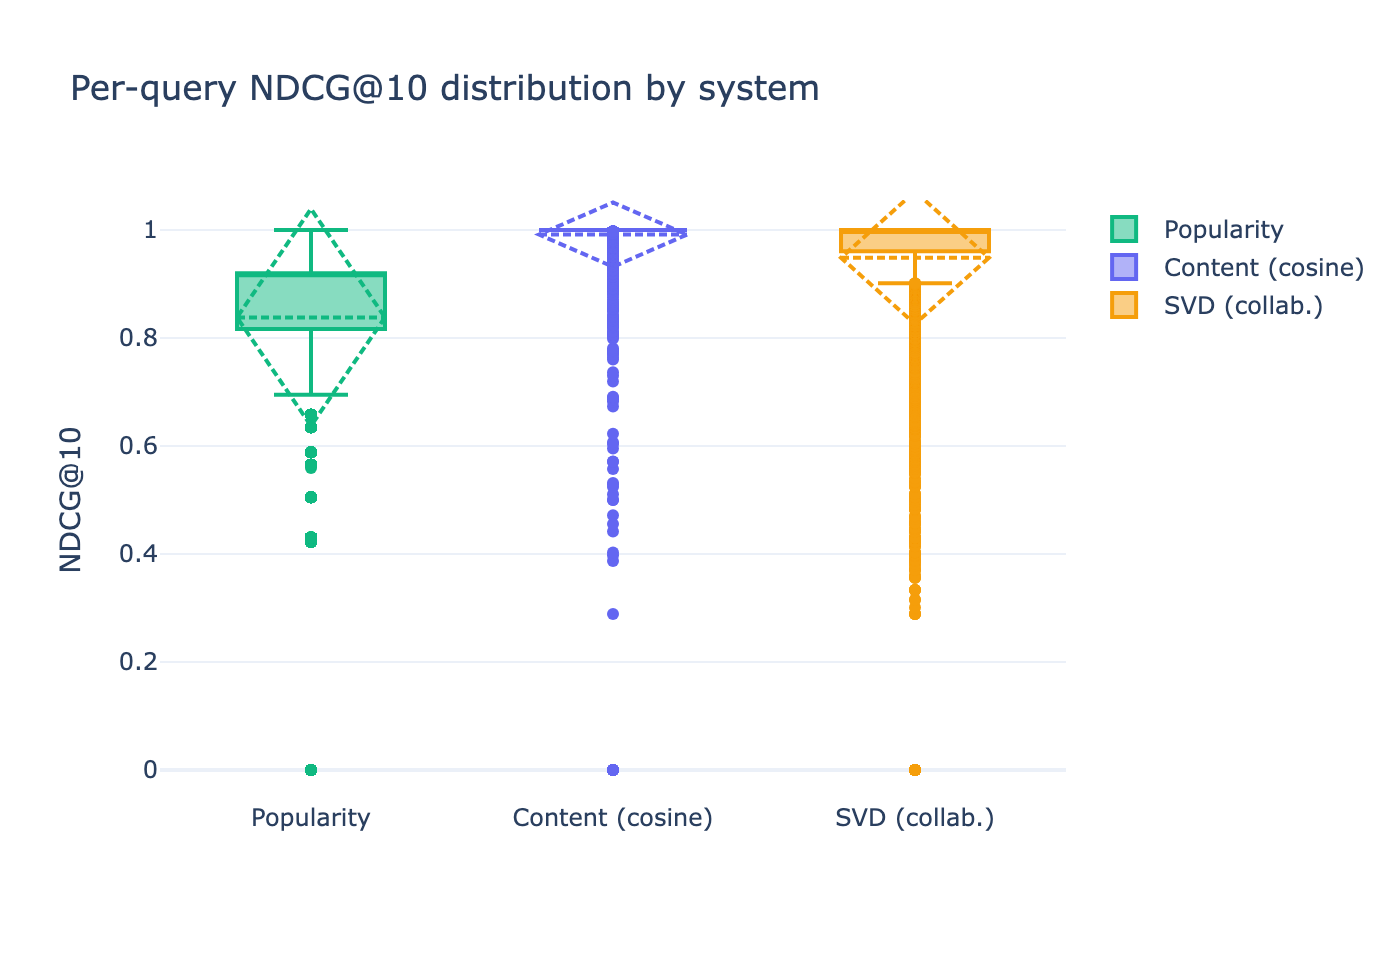
\includegraphics[width=0.85\textwidth]{../../artifacts/week10/week10_ndcg10_distribution.png}
  \caption{Box plots of per-query NDCG@10 for each system.
  Content cosine has the highest median and tightest spread.
  Popularity global shows the widest variance: its performance depends entirely on
  whether the query genre overlaps with the global top-100.}
  \label{fig:ndcg10_dist}
\end{figure}

%% ------------------------------------------------------------------
\section{Leave-One-Out (LOO) Evaluation}
\label{sec:loo}
%% ------------------------------------------------------------------

To complement the genre-based protocol, a second evaluation was conducted using
user rating histories from \texttt{ratings\_clean.parquet}.

\subsection{Protocol}

\begin{itemize}[nosep]
  \item Users with $\geq 5$ ratings; 10,000 sampled (\texttt{seed=42}).
  \item Last item by timestamp hidden as test; remainder used as training history.
  \item Each system recommends top-$K$ items excluding already-seen movies.
  \item Primary metrics: \textbf{Hit Rate@$K$} (equivalent to Recall@$K$ with one test item per user)
    and \textbf{NDCG@$K$}.
\end{itemize}

\textit{Note on Precision@$K$ in LOO:} with a single test item per user,
$\text{Precision@}K = \text{Hit Rate@}K / K$ by definition and carries no additional information.

\subsection{Results}

\begin{table}[H]
\centering
\caption{Leave-One-Out evaluation results ($n = 10{,}000$ users, \texttt{seed=42})}
\label{tab:loo_results}
\begin{tabular}{lcccc}
\toprule
\textbf{System} & \textbf{Hit Rate@5} & \textbf{Hit Rate@10} & \textbf{Hit Rate@20} & \textbf{NDCG@10} \\
\midrule
\texttt{popularity\_global}  & 0.0287 & 0.0465 & 0.0767 & 0.0238 \\
\texttt{content\_cosine}     & 0.0219 & 0.0368 & 0.0563 & 0.0187 \\
\texttt{svd\_collaborative}  & \textbf{0.0515} & \textbf{0.0795} & \textbf{0.1221} & \textbf{0.0432} \\
\bottomrule
\end{tabular}
\end{table}

Source: \texttt{artifacts/week10/week10\_loo\_evaluation\_results.csv} (\texttt{seed=42};
$n_{\text{queries}} = 10{,}000$ for popularity, 9,885 for content/SVD --- see the
candidate-pool definition in Section~\ref{subsec:candidate_pools}).
\texttt{cluster\_popularity} is not in this table: the LOO protocol requires the raw user
histories (\texttt{ratings\_clean.parquet}), which are reproducible from the Week~3 pipeline
but not committed to the repository; re-running the LOO notebook with a per-user
cluster-restricted pool is documented as follow-up work in Section~\ref{sec:worked}.

\paragraph{Key finding.}
\texttt{svd\_collaborative} \textbf{reverses the ranking} seen in the genre-based evaluation:
it achieves nearly double the Hit Rate@10 of Popularity (7.95\% vs.\ 4.65\%) and more than
double that of Content cosine (3.68\%). This confirms that SVD captures genuine behavioral
predictive signal, while content-based similarity is stronger for catalog discovery but
weaker at predicting individual user consumption.

The contrast also validates the Recall correction: the genre-based Recall@20 for
\texttt{content\_cosine} was $0.9994$ (inflated by the pool-denominator defect),
while the real retrieval rate under LOO is $5.6\%$.

\begin{figure}[H]
  \centering
  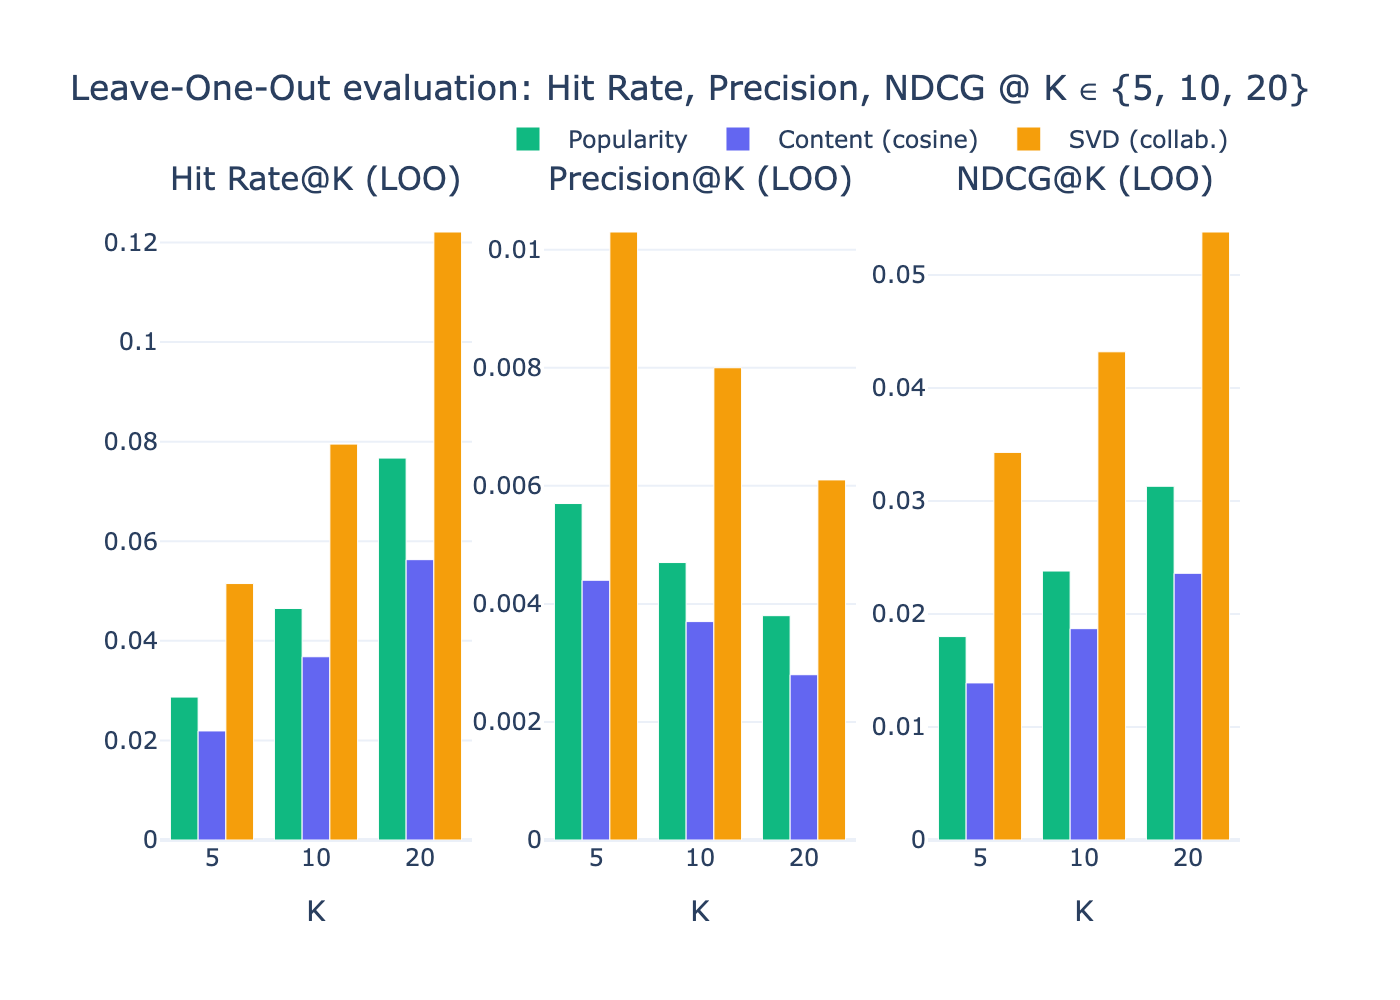
\includegraphics[width=\textwidth]{../../artifacts/week10/week10_loo_evaluation_comparison.png}
  \caption{LOO evaluation: Hit Rate, Precision, and NDCG at $K \in \{5, 10, 20\}$.
  SVD collaborative leads across all metrics; the reversed ranking relative to the genre protocol
  reflects its stronger user-behavior predictive power.}
  \label{fig:loo_comparison}
\end{figure}

%% ------------------------------------------------------------------
\section{Error Analysis}
%% ------------------------------------------------------------------

\subsection{Strong cases (Precision@10 = 1.0)}

\begin{table}[H]
\centering
\caption{Representative strong-case examples from the error analysis}
\begin{tabular}{p{3.2cm}p{4.8cm}p{3cm}p{3.5cm}}
\toprule
\textbf{System} & \textbf{Query movie} & \textbf{Genres} & \textbf{Reason} \\
\midrule
popularity\_global & Money Train (1995) & Action|Comedy|Crime|Drama|Thriller & Multi-genre query overlaps with mainstream top-100 \\
popularity\_global & Dead Presidents (1995) & Action|Crime|Drama & Same \\
content\_cosine & Toy Story (1995) & Adventure|Animation|Children|Comedy|Fantasy & Tight animation cluster in AE space \\
content\_cosine & Grumpier Old Men (1995) & Comedy|Romance & Dense comedy-romance neighborhood \\
svd\_collaborative & GoldenEye (1995) & Action|Adventure|Thriller & Strong user co-occurrence in Action/Thriller \\
svd\_collaborative & Tom and Huck (1995) & Adventure|Children & Clear behavioral cluster among family films \\
\bottomrule
\end{tabular}
\end{table}

\subsection{Failure cases (Hit Rate@10 = 0)}
\label{subsec:failures}

\begin{table}[H]
\centering
\caption{Representative failure cases from the error analysis}
\begin{tabular}{p{3.2cm}p{5cm}p{2.2cm}p{3.5cm}}
\toprule
\textbf{System} & \textbf{Query movie} & \textbf{Genres} & \textbf{Root cause} \\
\midrule
popularity\_global & Heidi Fleiss: Hollywood Madam (1995) & Documentary & Top-100 contains no documentaries \\
popularity\_global & Anne Frank Remembered (1995) & Documentary & Same \\
content\_cosine & Fair Game (1995) & Action & Embedding conflates with non-Action neighbors \\
content\_cosine & Repo Man (1984) & Comedy|Sci-Fi & Mixed-genre embedding pulls to wrong cluster \\
svd\_collaborative & Showgirls (1995) & Drama & Anomalous rating pattern; item factors incoherent \\
svd\_collaborative & Wyatt Earp (1994) & Western & Few Western films in filtered matrix; noisy factors \\
\bottomrule
\end{tabular}
\end{table}

\paragraph{Pattern.} Popularity global fails systematically for any genre underrepresented in
the global top-100 (Documentary, Western, Musical, Film-Noir). Content and SVD fail on edge cases:
genre-ambiguous films or items with few ratings.

The corrected evaluation (Section~\ref{subsec:corrected_table}) adds a hybrid-specific
failure mode: \texttt{cluster\_popularity} fixes the popularity baseline's niche-genre
failure \emph{when the niche has its own cluster} (Documentary queries now draw from
Cluster~5, which is 99.9\% documentaries), but inherits a new one --- queries whose genre is
a minority within their cluster get recommendations matching the cluster's majority genres
instead, which is why its Hit Rate@10 (0.821) is below the global baseline's (0.972).

%% ------------------------------------------------------------------
\section{What Worked and What Did Not}
\label{sec:worked}
%% ------------------------------------------------------------------

\paragraph{What worked.}
\begin{itemize}[nosep]
  \item The AE embedding space from Week~7 transfers cleanly to item-to-item recommendation,
    achieving Precision@10 = 0.978 --- near-perfect genre-relevant retrieval.
  \item SVD collaborative adds behavioral signal absent from content features:
    it correctly clusters behavioral co-occurrences even for genre-pure niche films.
  \item The cluster layer from Week~7 provides measurable signal: the
    \texttt{cluster\_popularity} hybrid is the more precise popularity baseline at $K=20$
    (0.578 vs 0.460) and solves the niche-genre failure for genres with their own cluster
    (Section~\ref{subsec:failures}).
  \item The evaluation protocol is fully reproducible without user-level ground truth ---
    and the corrected metrics can be recomputed from committed artifacts alone
    (\texttt{scripts/build\_week10\_eval\_corrected.py}), with a built-in reproduction check
    against the original run.
\end{itemize}

\paragraph{What did not work.}
\begin{itemize}[nosep]
  \item \textbf{Popularity global}: systematically fails for Documentary, Western, Musical,
    and Film-Noir --- any genre underrepresented in the global top-100 will receive zero
    relevant recommendations.
  \item \textbf{SVD coverage}: 45,871 movies (77.7\% of the catalog) are excluded from the
    filtered matrix ($<50$ ratings). Their item factors would be too noisy to produce
    meaningful recommendations.
  \item \textbf{Genre-based evaluation}: favors content methods by construction. SVD discovers
    behavioral patterns that may be more useful to users even when genres don't align perfectly.
  \item \textbf{Original Recall/NDCG implementation}: both metrics were self-referential
    (denominators derived from the system's own output). Corrected by recomputation; legacy
    values retained in Section~\ref{subsec:legacy_table} for traceability.
  \item \textbf{Hybrid under LOO (follow-up)}: evaluating \texttt{cluster\_popularity} under
    the LOO protocol requires regenerating \texttt{ratings\_clean.parquet} (Week~3 pipeline)
    and re-running the LOO notebook with a cluster-restricted candidate pool; left as
    documented follow-up work.
\end{itemize}

%% ------------------------------------------------------------------
\section{Ethics and Access Note}
%% ------------------------------------------------------------------

\begin{itemize}[nosep]
  \item \textbf{Data source}: GroupLens MovieLens~25M public release (research license).
  \item \textbf{Access}: Educational and research use; raw data not redistributed.
  \item \textbf{Personal data risk}: all user identifiers are anonymized integer IDs.
  \item \textbf{Mitigation}: all analysis at the movie level.
    SVD item factors are aggregate representations that do not expose individual user behavior.
\end{itemize}

%% ------------------------------------------------------------------
\section{Reproducibility}
%% ------------------------------------------------------------------

Notebooks must be run in this order:
\begin{enumerate}[nosep]
  \item \texttt{notebooks/week10/week10\_baseline\_recommender.ipynb}
  \item \texttt{notebooks/week10/week10\_matrix\_factorization.ipynb}
  \item \texttt{notebooks/week10/week10\_offline\_evaluation.ipynb}
\end{enumerate}

Then run the corrected evaluation (works from committed artifacts alone --- no raw data needed):

\begin{lstlisting}[language=bash]
python3 scripts/build_week10_eval_corrected.py
\end{lstlisting}

The script validates itself by reproducing the original legacy metrics (it aborts if the
maximum absolute difference exceeds 0.002) before writing
\texttt{week10\_genre\_eval\_corrected.csv}, \texttt{week10\_data\_alignment.csv}, and the
\texttt{genre\_eval\_corrected} block of \texttt{week10\_evaluation\_summary.json}.

All outputs are saved to \texttt{artifacts/week10/} ($\approx$40\,MB total).

\begin{table}[H]
\centering
\caption{Key parameters for reproducibility}
\begin{tabular}{ll}
\toprule
\textbf{Parameter} & \textbf{Value} \\
\midrule
Catalog size & 59,047 movies \\
Global mean rating $\mu$ & 3.0714 \\
Bayesian prior $C$ & 1.0 \\
Embedding dimension & 13 \\
Clusters ($k$) & 7 \\
SVD min. movie ratings & 50 \\
SVD min. user ratings & 20 \\
SVD $n\_\text{components}$ & 50 \\
SVD explained variance & 17.79\% \\
Matrix dimensions & 162,540 users $\times$ 13,176 movies \\
Matrix density & 1.15\% \\
Random state & 42 \\
\bottomrule
\end{tabular}
\end{table}

%% ------------------------------------------------------------------
\section{Conclusion}
%% ------------------------------------------------------------------

Week~10 is complete. Four recommendation systems --- two popularity baselines (one of them a
segmentation-fed hybrid), a content-based baseline, and an advanced collaborative model ---
were built, evaluated, and compared under two complementary protocols:

\paragraph{Genre-relevance evaluation, corrected (item-to-item, 4,994 queries --- Section~\ref{subsec:corrected_table}).}
\begin{itemize}[nosep]
  \item \textbf{Content cosine} (corrected NDCG@10 = \textbf{0.980}) is the strongest system
    for catalog discovery, leveraging the dense autoencoder embedding space from Week~7.
  \item \textbf{SVD collaborative} (corrected NDCG@10 = 0.872) ranks second, capturing
    behavioral co-occurrence patterns absent from content features.
  \item \textbf{Popularity global} (corrected NDCG@10 = 0.585) is the weakest at depth; the
    \textbf{cluster popularity hybrid} trades hit coverage for depth-stable precision and is
    the better popularity baseline at $K=20$ --- evidence that the Week~7 segmentation feeds
    the ranking with real signal.
\end{itemize}

\paragraph{Leave-One-Out evaluation (user history, 10,000 users --- Section~\ref{sec:loo}).}
\begin{itemize}[nosep]
  \item \textbf{SVD collaborative} (Hit Rate@10 = \textbf{7.9\%}) wins clearly,
    nearly doubling Popularity (4.6\%) and more than doubling Content cosine (3.7\%).
  \item This reversal reveals that SVD is the stronger \emph{predictive} model for user
    behavior, while content similarity is better for catalog discovery.
  \item The Recall@$K$ and NDCG@$K$ defects in the original genre protocol were identified,
    documented, and \textbf{corrected by recomputation}
    (Sections~\ref{subsec:relevance} and~\ref{subsec:corrected_table}), with the legacy
    numbers retained for traceability.
\end{itemize}

In rubric terms (Section~\ref{sec:framing}): the project is an \textbf{item-to-item
recommendation system operationalized as ranking}, with \textbf{segmentation feeding ranking}
in the hybrid baseline and a \textbf{prediction}-framed second protocol. The recommendation
layer is now a functioning component of the MovieLens Discovery pipeline, and the cluster
segmentation from Week~7 sets up the graph analytics layer in Week~12.

\end{document}
